In the original article where the terminology ``Debt-trap Diplomacy'' was coined, \citet{Chellaney_2017} specifically mentioned the predicament faced by the Sri Lankan government. He argues that the Chinese government supported large infrastructure projects in Sri Lanka and provided heavy loans to their government, and as the project eventually failed to repay the debt, the country is then ensnared in the concessions to China. \autoref{fig: sri-lanka-debt-ts} shows the change in composition of the creditors to Sri Lanka.

The issue of the Hambantota port is regarded as a typical example of a debt-trap for some scholars~\citep*{Moramudali_2020}.
The construction of the port was initiated in 2007 and entrusted to the state-owned Chinese companies --- China Harbour Engineering Company and Sinohydro Corporation. The project was valued at \$361 million, of which Exim Bank financed 85\% at a yearly interest rate of 6.3\%\footnote{From AidData Project ID \#33409, ``China Eximbank provides \$306.7 million buyer's credit loan for Phase I of Hambantota''}.


China's involvement in Sri Lanka's infrastructure development was facilitated by President Mahinda Rajapaksa, during which China became Sri Lanka's leading investor and lender. This gave China significant diplomatic leverage over Sri Lanka. 
However, when Rajapaksa was unexpectedly defeated in the early 2015 election by Maithripala Sirisena, who campaigned on the promise to extricate Sri Lanka from the Chinese debt trap, work on major Chinese projects was suspended.

However, Sri Lanka's government was already on the brink of default, and Sirisena eventually acquiesced to a series of Chinese demands\footnotemark{}, including the sale of an 70\% stake in the Hambantota port to China Merchants Port (CM Port) and a 99-year lease.
\footnotetext{This narrative origins from \citet*{Chellaney_2017}. \citet*{Brautigam-meme-2020}, however, provides a different narrative. She mentioned that ``\emph{The proceeds were used to increase Sri Lanka's
US dollar reserves in 2017-18 with a view to the repayment of maturing international sovereign bonds \dots Therefore, the sale of Hambantota was originally a fire sale designed to raise money to deal
with larger debt problems.}''}
Notably, as argued by \citet*{Moramudali_2019}, the lease did not write off the loans obtained to construct Hambanota port. The proceeds from the lease were used to boost the country's dollar reserves in 2017-18, especially in preparation for the large amount of external debt that needed to be serviced when international sovereign bonds matured in early 2019. This means that the lease is not a debt-equity-swap, as common narratives elaborated \citep*{Moramudali_2020}.
Sri Lanka eventually declared a suspension on payment on most foreign debt from Aril 12, 2022. Whether Sri Lanka was indeed already under the extreme ``brink of default'' during 2015 is a major gap in the literature of sovereign default that has not yet been investigated.

\begin{figure}[t!]
    \centering
    \begin{subfigure}[position]{0.48\textwidth}
        \centering
        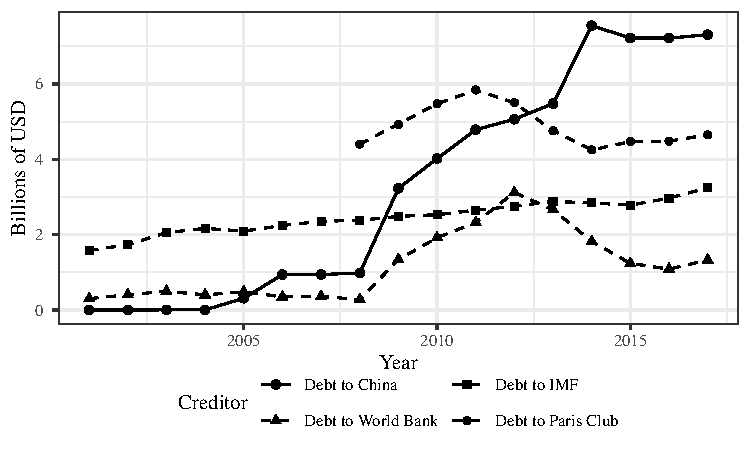
\includegraphics[width=\textwidth]{fig/ALL/Sri Lanka_debt_source.pdf}
        \caption{Sri Lanka}
        \label{fig: sri-lanka-debt-ts}
    \end{subfigure}
    \begin{subfigure}[position]{0.48\textwidth}
        \centering
        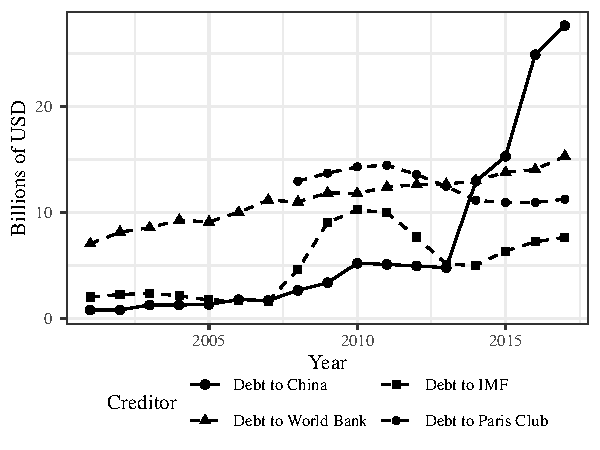
\includegraphics[width = \textwidth]{fig/ALL/Pakistan_debt_source.pdf}
        \caption{Pakistan}
        \label{fig: pakistan-debt-ts}
    \end{subfigure}
    \caption{Debt to All Creditors}
    \floatfoot{Source: HRT Database \citeyearpar{Horn-Reinhart-Trebesch-21} \\
    Note: The figure shows the change in the external public debt that Sri Lanka and Pakistan owed to different official creditors. These include China, World Bank (excluding China), IMF, and all 22 Paris Club governments.}
\end{figure}